\chapter{Research methodology}

The aim of this research is to produce a technology-based solution to the problem of non-contact emotion detection within the context of games research. The solution is a software composed of a user-tailored model that is trained from a game-based calibration phase and is able to infer the emotional state of a player regarding stress and boredom via analysis of remotely acquired user signals. The contructs, models and methods involved in such aim have been individually studied in previous research, however the combination of all those elements in a single solution within the context of games research is novel. The utilization of those elements in combination is not yet proved to work, so an iterative and incremental process must be conducted to identify challenges, problems and solutions to achieve the desired goal.

\begin{figure}[h]
    \centering
    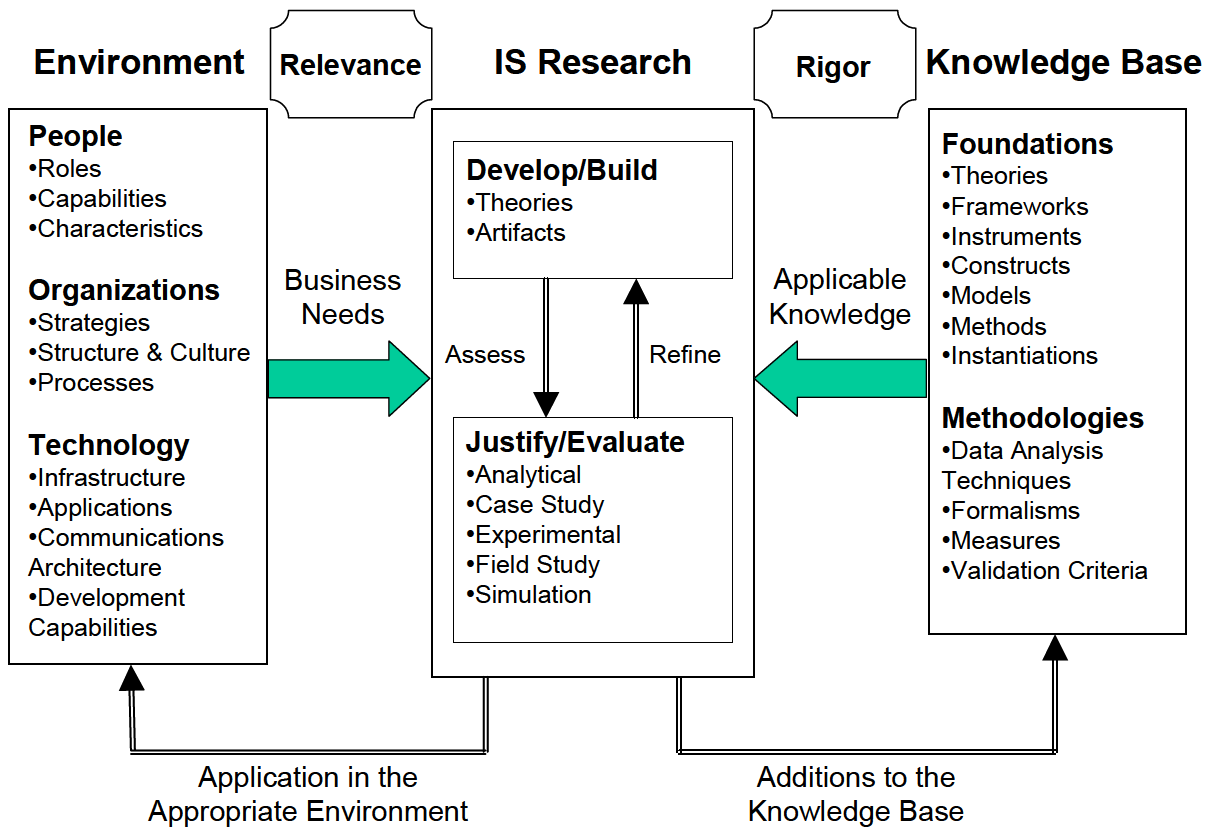
\includegraphics[width=\textwidth]{figures/hevner-research-framework.png}
    \caption{A framework for design science in the context of Information Technology \parencite{hevner2004design}}
    \label{fig:hevner-research-framework}
\end{figure}

A research methodology that fits such iterative process is design science. As defined by \textcite{hevner2004design} and illustrated in Figure \ref{fig:hevner-research-framework}, design science is a problem solving process that explores a relevant problem within an environment, iteratively measuring and refining the proposed solution according to the existing body of knowledge. The progress is made iteratively as the scope of the design of the artifact is expanded based on the discovery of available means, ends and constraints.

The use of a game-based calibration phase in this research influences how users behave during the emotion elitication process, e.g. body movement and facial expression. The movement of users directly impact the techniques for remote extraction of user signals during both the calibration phase and the emotion estimation phase, since those techniques are highly influenced by motion. The accuracy of those techniques regarding the remotely acquired signals is affected as well, which might invalidate the feasibility of remotely reading determined physiological and non-physiological signals required by the emotion estimaion model. The computer vision techniques, the model and the process associated with them must be continuously investigated and adapted to overcome those challenges. As a consequence, an iteractive cycle of development and research is required, as illustrated by Figure \ref{fig:hevner-generate-test}. In each iteration, a possible solution for the current set of problems is generated, rigourly tested and evaluated, producing information to guide the next iterations in the cycle. The set of design alternatives in this research are related to the identification of physiological and non-physiological signals to be used in the emotion detection process, how they can be elicitated with games in a calibration phase, which computer vision techniques can be employed to remotely acquire the signals and which machine learning model is able to map the information into emotional states. The set of constraints involve problems associated with user behaving naturally, e.g. laughing and moving the body during the procedure, use of non-specialized hardware, e.g. ordinary camera, accuracy and efficienty of the solution, among others.

\begin{figure}[h]
    \centering
    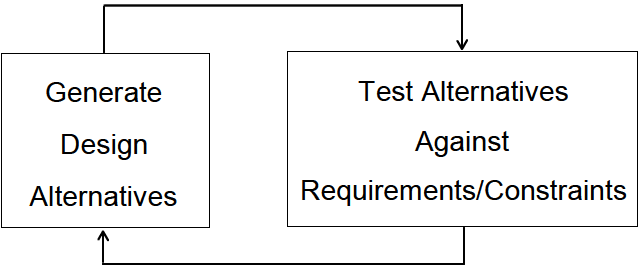
\includegraphics[width=0.6\textwidth]{figures/hevner-generate-test.png}
    \caption{The Generate/Test cycle. Adapted from \textcite{hevner2004design}}
    \label{fig:hevner-generate-test}
\end{figure}

%The aim of this research is to produce a utility tool, i.e. software, which is an artifact based on a model built on existing theories, which will be combined in a new and innovative way. Since the result of the research is a model, which will be built from different measurements to predict or infer a state, the present work stands on the positivism paradigm. Essentially this work will formulate a theory about how the variation of physiological signals relate to stress/boredom levels in the context of games and how it can be remotely detected. The involvement of humans in the process might relate to the social side of interpretivism, however the foundation of the work is still based on the analysis of physiological signals. Such signals and their patterns might be different for each person, however they are still ordered and regular under the human being perspective. As a consequence, they can be objectively observed, measured and analysed with a quantitative approach and hypothesis testing.

Design-science research requires the application of rigorous methods in both the construction and evaluation of the designed artifact \parencite{hevner2004design}. One of the such evaluation methods is experimental research, which is the strategy used to build and validate the knowledge in this project. Such approach is composed of a set of research designs that use controlled testing and manipulation of variables in order to understand casual processes. The foundation of an experiment is to manipulate a variable (or a set of them) and measure any changes in other variables. It establishes the effect on a dependent variable, which is the focus of the research. The model being constructed in this research links the variations of physiological signals to stress/boredom levels in the context of games, hence there is a causal effect in the process since identified variations (cause) will precede changes in stress/boredom levels (effect). It progresses to the construction of a hypothesis where the cause will consistently lead to the same effect so the link between variations of signals and emotional levels can be inferred or predicted.

Each iteration in the design of the artifact will be constructed based on systematical investigation of existing theories, which will be refined and adapted to the context of the artifact. An experiment will validade the current artifact, producing information to guide the next iteration. The following section detail how the research will be conducted and what is the current state of the project.

%\section{Research objectives}

%The objective of this research is to produce a method that is able to interpret remotely acquired signals from a person playing a game and detect his/her current emotional state regarding stress and boredom according to data previously obtained in a calibration phase. The model will be implemented in a software that uses a video feed to detect the person's emotional state.

%The current approaches used to obtain information from the players during games research inevitably affect the player's experience. They require the user to stop the game activity in order to share his/her current state, such as by answering a questionnaire. The frequency that such questionnaires are issued is also a concern. If performed too often, more information might be collected, but the data might contain noise caused by the frequent interruptions, e.g. player is more stressed/bored by the questionnaire interruptions than by the game itself. If performed too sparse, not enough information will be gathered from the player. A physical sensor attached to a player, on the contrary, allows a continuous monitoring process, however it is intrusive and might interfere with the player capacity to interact with the game. It might prevent the use or movement of specific parts of the body, for instance. Physical sensors also increase the chances of the player to behave differently as a side-effect of the monitoring process itself.

%A purely remote-based solution, as the one proposed by this research, enhances the tooling available to the games research community regarding investigation methods of stress and boredom. A games researcher will be able to increase the internal validity of his/her workflow by ensuring the player keeps the focus on the game without interruptions and by minimizing the side effects (and inconveniences) of physical monitoring. This research could also be deployed as a solution for game developer studios to automatically analyze hours of recorded gameplay and highlight the moments when boredom/stress levels changed significantly. As a complement the solution will be based on a single, ordinary camera and a software implementation, which eliminates the use of complex setups of physical sensors. It eases the investigation process and reduces costs.

\section{Current state of research}

As previously mentioned, this research is based on an interative problem solving strategy that involves the investigation and evaluation of different components. Figures \ref{fig:user-tailored-calibration} and \ref{fig:user-tailored-use}, in section \ref{sec:research-aim}, illustrate the combined use of the different parts involved in this project, which are all connected to the research objectives presented in section \ref{sec:contributions}. Figure \ref{fig:components-objectives} illustrates the correlation among the research objetives and the parts required to achieve the proposed research aim.

\begin{figure}[h]
    \centering
    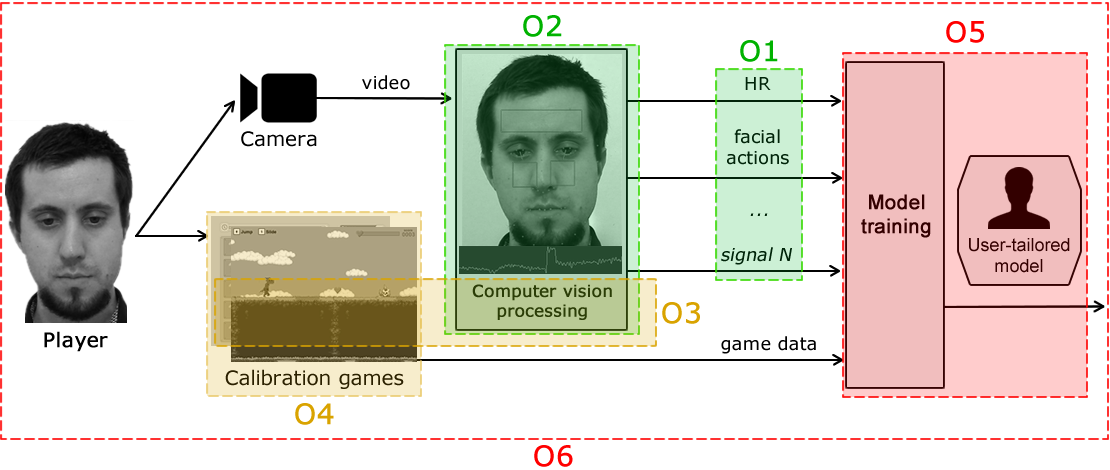
\includegraphics[width=\textwidth]{figures/components-objectives.png}
    \caption{Correlation among the research objetives and the parts required to achieve the proposed research aim. Red labels: not fulfilled yet. Yellow labels: partially fulfilled. Green labels: completely fulfilled.}
    \label{fig:components-objectives}
\end{figure}

Objectives marked in red and yellow are not fulfilled and partially fulfilled, respectively, so more investigation will be conducted regarding them. For information regarding future work, refer to chapter \ref{ch:closing}. Objectives marked in green have already been fulfilled and the theories, concepts and results associated to each of them is documented in this thesis proposal. The chapters where such documentation and the associated objectives exist in this thesis is presented in Figure \ref{fig:research-current-state}.

%The experiment design will be based on a within-subject approach \cite{lane2015online}. In such approach, all participants perform at all levels of the treatment and there are no control groups. It is the opposite of a between-subjects approach, where subjects are divided in more than one group that receive different treatments. In that approach there are special groups, called control groups, that receive no treatment. The comparison between the control groups and the treatment groups ensures internal validity. In the context of this research, physiological signals will be measured, so the division of subjects into more than one group poses a comparison problem. Each individual will inevitably differ from one another regarding physiological signals, such as variations in average HR during rest, for instance. When measuring HR, for instance, some subjects will have higher/lower HR mean than others, independent of the group they are in or the treatment they undergo. To counter that problem, the experiment will use a one-group posttest design \cite{kirk1982experimental}, as illustrated by Figure \ref{fig:experiment}. Using the first row as an example, subject $S_0$ played game $G_a$ as the first level of the treatment, followed by a post-test of that game ($PT_a$), then a rest period. In the second level of the treatment, the subject played game $G_b$, followed by a post-test of that game ($PT_b$), then another rest period. Finally in the third level of the treatment, the subject played game $G_c$ followed by a post-test of that game ($PT_c$).

%\begin{figure}[ht]
%    \centering
%    \includegraphics[scale=0.5]{imgs/experiment-design.png}
%    \caption{One-group posttest experiment design used in this research. $S_j$ represents the $j^{\text{th}}$ subject, $G_i$ represents a game of type $i$, $PT_i$ is the post-test for game $G_i$ and $rest$ is a resting period.}
%    \label{fig:experiment}
%\end{figure}

%By using a one-group posttest design, each individual will perform on all levels of the treatment (play a set of different games). The within-subjects approach ensures that the differences between subjects are not interfering in the comparison, since a subject is being compared to his/herself in the different levels of the treatment. Subjects are not being compared among each other. In essence, each subject is serving as his/her own control group. According to Kirk \cite{kirk1982experimental}, the one-group posttest design should only be used when the researcher knows the mean value of the independent variable when no treatment is in effect. Such information will be obtained during the resting periods of the experiment, where the baseline value for all measured signals can be established for each subject.

%The process of sampling a group of participants for each experiment will follow the convenience sampling approach, a non-probability sampling technique where participants are recruited because of their convenient accessibility/proximity to the researcher. Volunteers will be randomly recruited for each experiment. A probability sampling approach, where each individual of the population has an equal chance of being selected, would be ideal and would strength the external validity of the research. However the costs, logistics and time constraints associated with it makes such approach impractical in the context of this research.

Both objectives \textbf{O1} and \textbf{O2} have already been fulfilled. After the first literature review, the accomplishment of \textbf{O1} produced the identification of the main concepts, theories and signals associated with phychophysiological profile of users and their emotions. Chapters \ref{ch:literature-games}, \ref{ch:literature-physiological} and \ref{ch:literature-multifactorial} present the results of such literature review. The results of the literature review regarding objective \textbf{O2}, which focus on the identification of ideal existing computer vision techniques to remotely extract signals from users, is presented in chapters \ref{ch:literature-face} and \ref{ch:literature-rppg}. The investigation also produced a publication regarding emotion detection and remote measurement of physiological signals \parencite{bevilacqua2015proposal}.

\begin{figure}[ht]
    \centering
    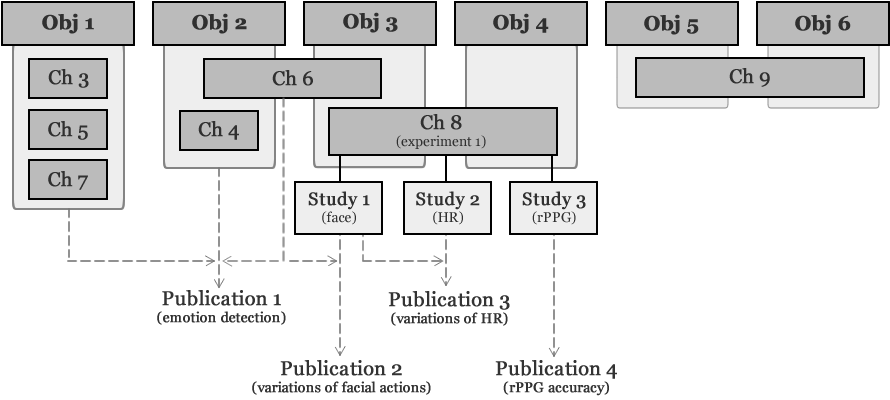
\includegraphics[width=\textwidth]{figures/research-current-state.png}
    \caption{The thesis chapters coupled with the research objetives they cover.}
    \label{fig:research-current-state}
\end{figure}

Objective \textbf{O3} is being finalized. The aim of that objective, which is the investigation of feasibility, accuracy and challenges regarding the application the computer vision techniques within the context of games, was performed as an experiment. The experiment and the three studies conducted on the collected data are described and presented in chapter \ref{ch:experiment1}. Each one of those studies resulted in a publication, which present results regarding variations of facial actions \parencite{bevilacqua2016variations}, variations of heart rate \parencite{bevilacqua2017changes} and accuracy evaluation of the selected computer vision technique \parencite{bevilacqua2017accuracy}. The last two aforementioned publications were recently submitted for review. The main challenges regarding the application of the computer vision techniques within the context of games have already been identified. A publication \parencite{bevilacqua2017accuracy} and the literature review presented in chapter \ref{ch:literature-rppg} show the limitations of the computer vision technique when applied to contexts of games research involving natural behavior of users, e.g. head movement and face oclusion. A new study will be conducted to investigate ways to improve the computer vision technique to eliminate or mitigate such limitations.

Objective \textbf{O4} has been partially fulfilled. A pilot study, an experiment (described in chapter \ref{ch:experiment1}) and two publications \parencite{bevilacqua2016variations,bevilacqua2017changes} describe and validate the concept of calibration games. Up to the present moment, however, the variation of the signals produced by such calibration games have not been employed in any studies or experiments involving emotion detection, so its utility within the context of this research needs to be further investigated.
